\documentclass[aspectratio=1610, 13pt]{beamer}
\usepackage{xcolor}
\usepackage{multicol}
\usepackage{mathtools,array}
\usepackage[T1]{fontenc}

\usepackage{stmaryrd}
\usepackage{dutchcal}
\usepackage{zi4}
\usepackage[font={scriptsize,bf}]{caption}
% \usepackage{subcaption}
\usepackage{graphics}
\usepackage{tikz}
\usepackage{fontawesome5}
\usepackage{mathpartir}

\newcommand{\naturals}{\mathbb{N}}
\newcommand{\reals}{\mathbb{R}}

\newcommand{\Dist}[1]{\mathcal{D}(#1)}
\newcommand{\expectation}{\mathbb{E}}

\newcommand{\states}{S}
\newcommand{\actions}{A}
\newcommand{\observables}{O}
\newcommand{\trans}{T}
\newcommand{\obs}{Z}
\newcommand{\reward}{R}
\newcommand{\discount}{\gamma}

\newcommand{\beliefs}{\mathcal{B}}
\newcommand{\beliefUpdate}{\tau}

\newcommand{\policy}{\pi}

\newcommand{\diff}[1]{\mathop{}\!\mathrm{d}#1}
\renewcommand{\figurename}{Figure}
\renewcommand{\refname}{Reference}

\AtBeginDocument{
  \catcode`_=12
  \begingroup\lccode`~=`_
  \lowercase{\endgroup\let~}\sb
  \mathcode`_="8000
}

% \usetheme{Madrid}
% % \usetheme{default}
% \setbeamertemplate{caption}[numbered]
% \setbeamerfont{title}{size=\large}
\mode<presentation>
{
  \usetheme{Darmstadt}      % or try Darmstadt, Madrid, Warsaw, ...
  \usecolortheme{default} % or try albatross, beaver, crane, ...
  \usefonttheme[onlymath]{serif}  % or try serif, structurebold, ...
  \setbeamertemplate{navigation symbols}{}
  \setbeamertemplate{caption}[numbered]
  \setbeamertemplate{footline}[frame number] 
} 

\usepackage{listings}
\lstdefinestyle{heaplang}{
    language=Caml,
    basicstyle=\footnotesize\ttfamily,
    keywordstyle=\color{blue},
    commentstyle=\color{red},
    escapeinside={<@}{@>},
    morekeywords={new_chan, fork, recv, send, swap, ref}
}
\lstdefinestyle{clang}{
    language=Caml,
    basicstyle=\footnotesize\ttfamily,
    keywordstyle=\color{blue},
    commentstyle=\color{red},
    escapeinside={<@}{@>},
}
\lstset{style=heaplang}

\usepackage{natbib}

\newcommand{\buchi}{B\"uchi }

\definecolor{goldenpoppy}{rgb}{0.99, 0.76, 0.0}
\definecolor{goldenyellow}{rgb}{1.0, 0.87, 0.0}
\definecolor{green2}{rgb}{0.1,0.7,0.3} 
\newcommand{\gcheck}{{\color{green2}\faCheckCircle[regular] }}
\newcommand{\rcross}{{\color{red} \faTimesCircle[regular]} }
\newcommand{\rflag}{{\color{red} \faFlag}}
% \usepackage{algorithm,amsmath}
% \usepackage[noend]{algpseudocode}

\newcommand{\zlstinline}{\let\par\endgraf\lstinline}
\newcommand{\comments}[1]{{\color{red}#1}}
\title{Lazy Abstraction \& Spatial Interpolant}
\author{Reporter:  Xie Li}
\date{\today}
\begin{document}
\maketitle
\begin{frame}{Papers}
\begin{itemize}
\item Lazy Abstraction with Interpolants. CAV'06
\item Spatial Interpolants. ESOP'15
\end{itemize}
\end{frame}

\begin{frame}{Example: Lazy Abstraction with Interpolants}
\begin{center}
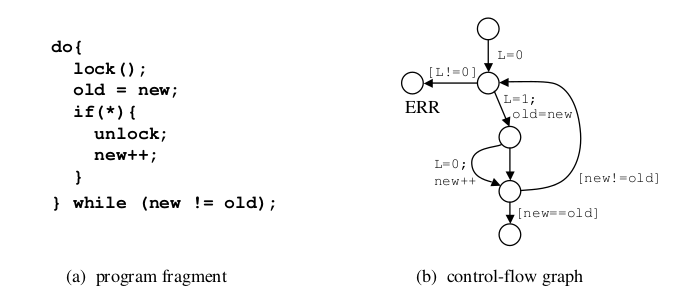
\includegraphics[scale=0.4]{0.png}
\end{center}

\texttt{L} is the variable for lock, locked if \texttt{L} $= 1$.

Prove: \texttt{L} is always $0$ on entry to \texttt{lock}. 

\begin{itemize}
\item 
Unwind the program into a tree, and label the true statements for each tree node.
\item Find a labeling that root is \textsc{True} and error states are \textsc{False}.
\end{itemize}

\end{frame}

\begin{frame}{Interpolants}
An interpolant  for $(A, B)$ is a formula $A'$ s.t.
\begin{itemize}
\item $A\rightarrow A'$
\item $A' \wedge B$ is unsatisfiable and 
\item $A' \in \mathcal{L}(A) \cap \mathcal{L}(B)$
\end{itemize}

We say $A_0', \ldots, A_n'$ is an interpolant for $\Gamma = A_1, \ldots, A_n$ when
\begin{itemize}
\item $A_0' = \textsc{True}, A_n' = \textsc{False}$
\item For all $ 1 \le i \le n, A_{i-1}'\wedge A_i\implies A_i'$
\item For all $ 1 \le i < n, A_i'\in \mathcal{L}(A_1\ldots A_i) \cap \mathcal{L}(A_{i+1}\ldots A_n)$
\end{itemize}
\end{frame}

\begin{frame}\frametitle{Example: Unwinding}

\begin{center}
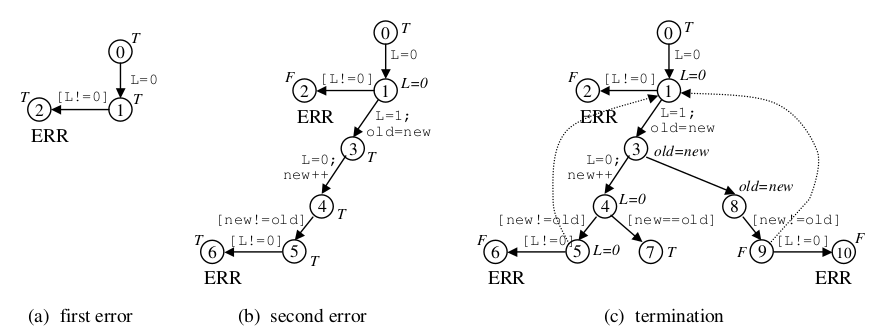
\includegraphics[scale=0.4]{2.png}
\end{center}
Dashed arrow represents the covering relation $\triangleright$. e.g. $(5,1)\in \triangleright$.


\end{frame}
\begin{frame}\frametitle{Formalization: Program}
\begin{itemize}
\item A program is a tuple $(\Gamma, \Delta, l_i, l_f)$. e.g. $(l, T, m)\in \Delta$, and $T$ is a transition formula.
\item A path $\pi$: $(l_0, T_0, l_1), (l_1, T_1, l_2), \ldots, (l_{n-1}, T_{n-1}, l_n)$. Error path.
\item The unfolding $\mathcal{U}(\pi)$ of a path: $T_0^{\langle 0\rangle}, \ldots, T_n^{\langle n-1\rangle}$
\item Inductive invariant: $I: \Lambda \rightarrow \mathcal{L}(S)$, s.t. $I(l_i) = \textsc{True}$ and for every $(l, T, m)\in \Delta
$, $I(l)\wedge T \rightarrow I(m)'$.

\item Safety invariant: An inductive invariant $I$ s.t. $I(l_f) = \textsc{False}$.
\end{itemize}
\end{frame}

\begin{frame}{Formalization: Unwinding}
\begin{center}
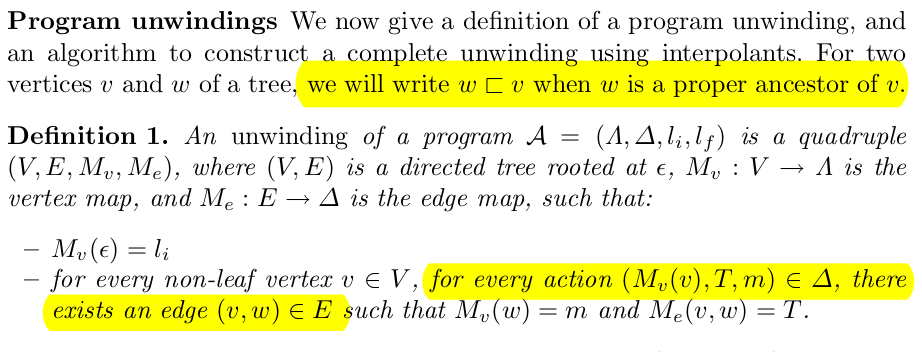
\includegraphics[scale=0.4]{3.png}
\end{center}
\end{frame}\begin{frame}{Formalization: Unwinding}
\begin{center}
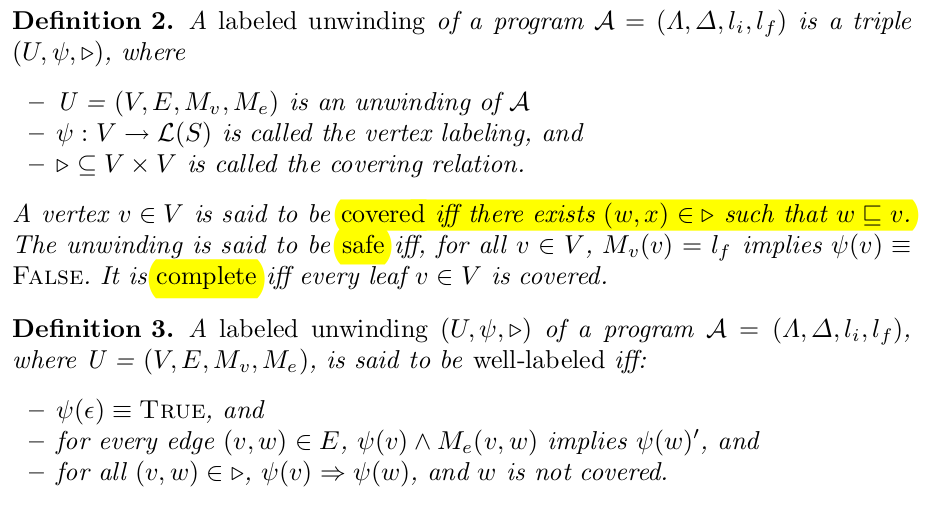
\includegraphics[scale=0.4]{4.png}
\end{center}
\end{frame}

\begin{frame}{Soundness}
\begin{theorem}[Soundness]
If there exists a safe, complete, well-labeled  unwinding of program $\mathcal{A}$, then $\mathcal{A}$ is safe.
\end{theorem}
\begin{proof}
Let $U$ be the set of uncovered vertices, and let function $M$ map location $l$ to $\bigvee \{\psi(v)\mid M_v(v) = l, v\in U\}$. $M$ is a safety invariant for $\mathcal{A}$.
\end{proof}


\end{frame}

\begin{frame}{Algorithm}
\begin{center}
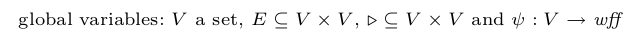
\includegraphics[scale=0.4]{5.png}

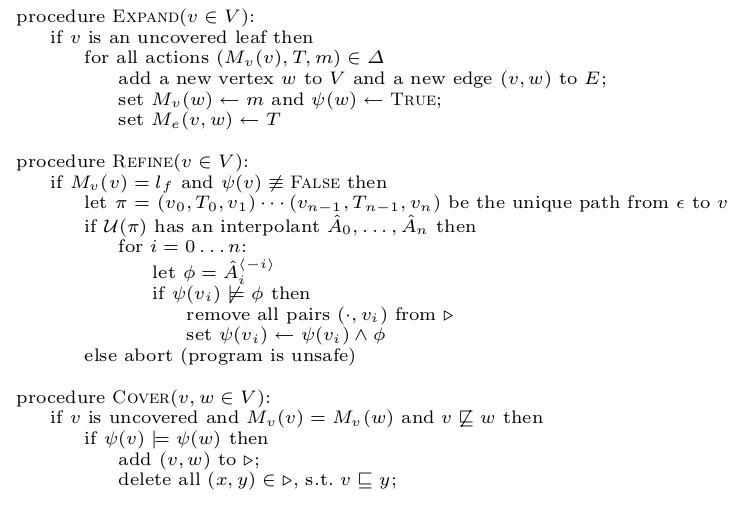
\includegraphics[scale=0.4]{6.png}
\end{center}
\end{frame}
\begin{frame}{Algorithm}
\begin{center}
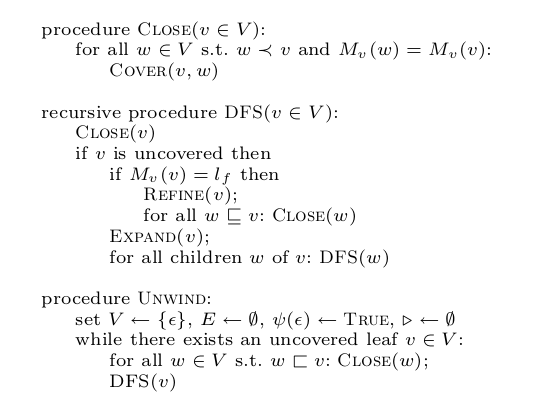
\includegraphics[scale=0.4]{7.png}
\end{center}
where $\prec$ is the relation regarding $\sqsubseteq $, indicating the order of computing  the covering relation. Since adding a new pair may delete old pairs.
\end{frame}

\begin{frame}{Lazy Abstraction with Spatial Interpolants}
Procedure:
\begin{itemize}
\item Sample a program path and construct a Hoare stype proof of this path.
\item Compute Spatial Interpolants
\item Refine with Theory Interpolants
\item From Proofs of Paths to Proofs of Programs
\end{itemize}
\end{frame}

\begin{frame}{Example: Spatial Interpolants}
\begin{center}
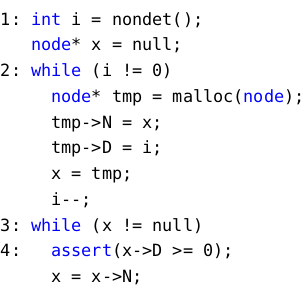
\includegraphics[scale=0.3]{8.png}

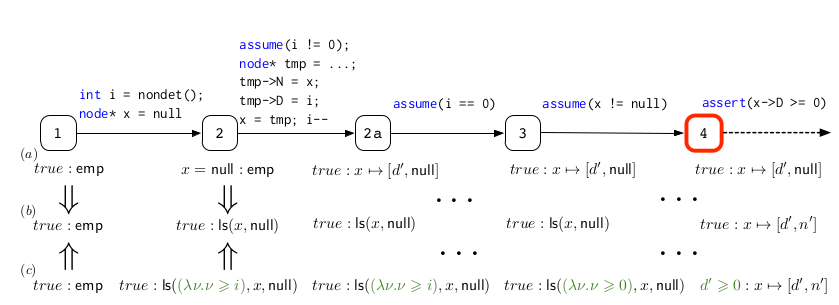
\includegraphics[scale=0.4]{9.png}
\end{center}
\end{frame}


\begin{frame}{Preliminaries: Separation Logic}
\begin{center}
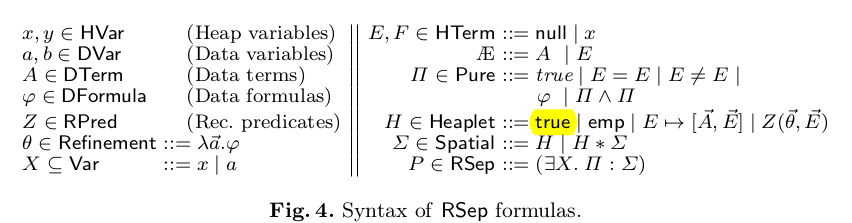
\includegraphics[scale=0.4]{10.png}
\end{center}
Features:
\begin{itemize}
\item General recursive predicates.
\item Recursive predicates are augmented with a vector of refinements on data values.
\item Each heal cell is a record consisting of data fields followed by heap fields.
\item Pure formulas contain heal and first-order data constraints.
\end{itemize}
\end{frame}

\begin{frame}{Preliminaries: Separation Logic}
Separation conjunction:
$$P \ast Q = (\exists X_P \cup X_Q. \Pi_P\wedge \Pi_Q : \Sigma_P \ast \Sigma_Q)$$

We write $\exists X. P$ to denote:
$$\exists X. P = \exists X\cup X_P. \Pi_P : \Sigma_P$$

Recursive predicates:
\begin{center}
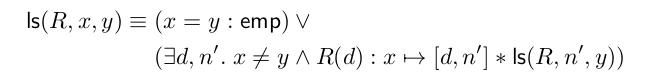
\includegraphics[scale=0.4]{11.png}

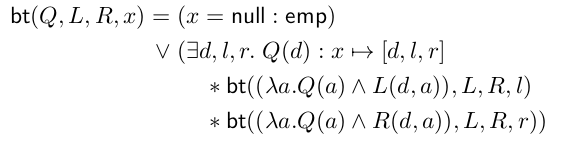
\includegraphics[scale=0.4]{12.png}
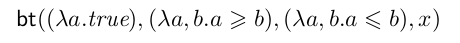
\includegraphics[scale=0.4]{14.png}
\end{center}
\end{frame}

\begin{frame}{Prelimiaries: Separation Logic}

Generally
\begin{center}
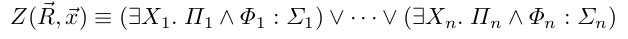
\includegraphics[scale=0.4]{13.png}\end{center}
Semantic of recursive predicates:
\begin{center}
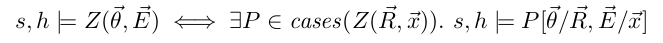
\includegraphics[scale=0.4]{15.png}
\end{center}
\end{frame}

\begin{frame}{Prelimiaries: Program}
Program is a tuple $\langle V, E, v_i, v_e\rangle$.

Each edge  $e\in E$ is connected with an edge command $e^c$.




\begin{center}
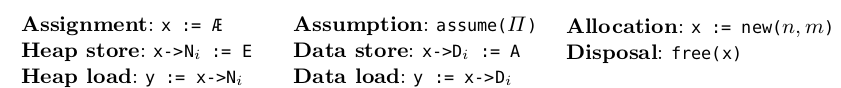
\includegraphics[scale=0.4]{16.png}
\end{center}
\end{frame}

\begin{frame}{Phase 1: Forward Symbolic Execution}
For heap statements:
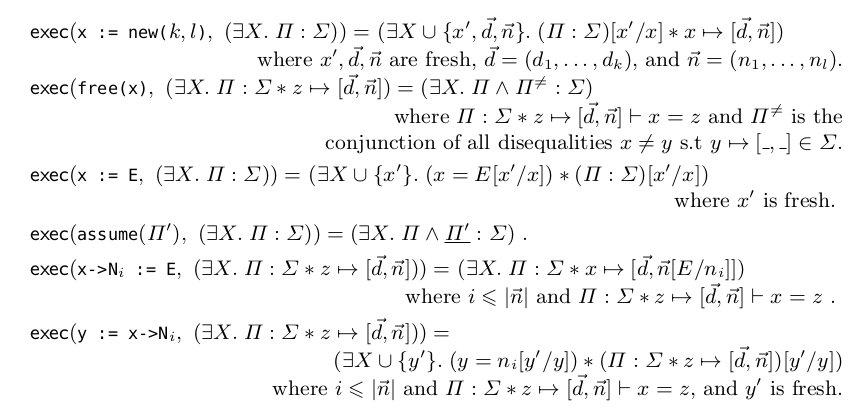
\includegraphics[scale=0.4]{17.png}
\end{frame}
\begin{frame}{Phase 2: Backward Interpolation Phase}
Spatial Interpolants:
\begin{center}

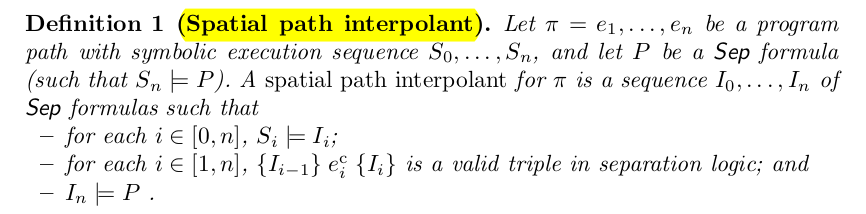
\includegraphics[scale=0.4]{18.png}
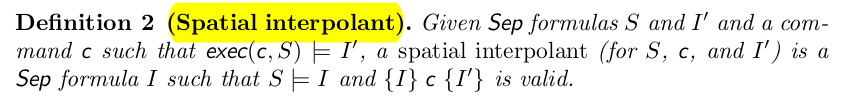
\includegraphics[scale=0.4]{19.png}
\end{center}


\end{frame}

\begin{frame}{Example Review}

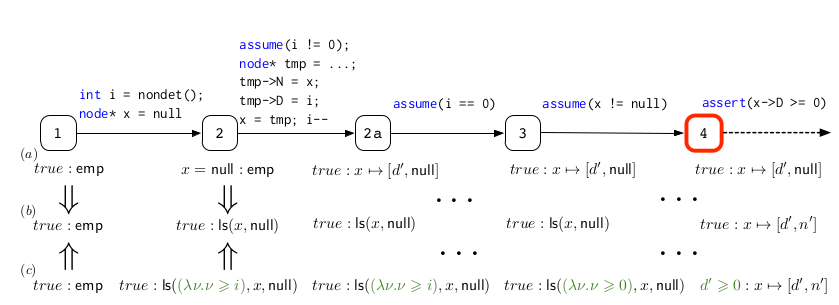
\includegraphics[scale=0.4]{9.png}
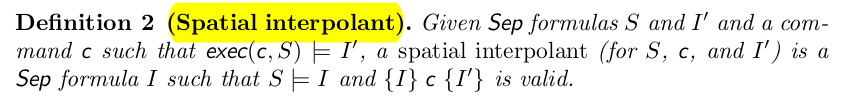
\includegraphics[scale=0.4]{19.png}
\end{frame}

\begin{frame}{Phase 2: How to Compute Spatial Interpolants}
\textbf{Bounded Abduction:}
\begin{center}

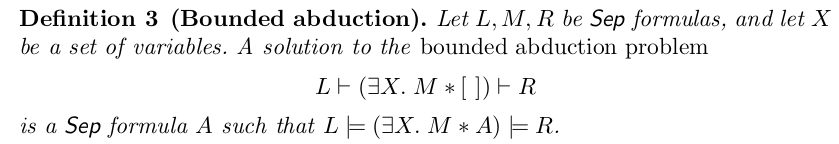
\includegraphics[scale=0.4]{20.png}
\end{center}
\end{frame}

\begin{frame}\frametitle{Bounded Abduction Rules}
\begin{center}
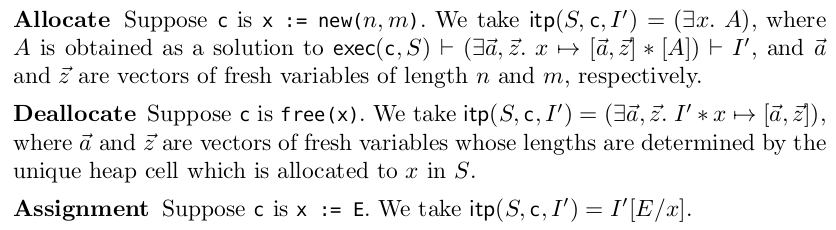
\includegraphics[scale=0.4]{21.png}
\end{center}
\end{frame}

\begin{frame}{Bounded Abduction Rules for Load and Store}
\begin{center}
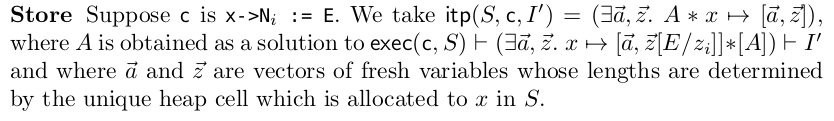
\includegraphics[scale=0.4]{22.png}
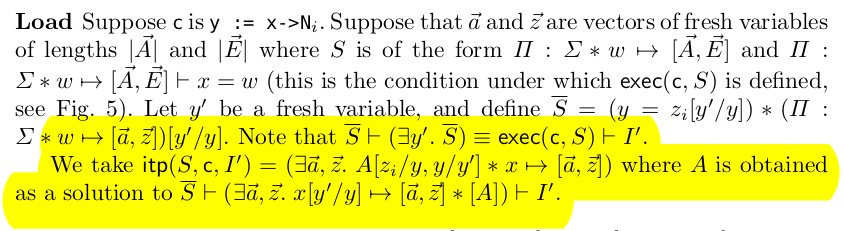
\includegraphics[scale=0.4]{23.png}
\end{center}
\end{frame}

\begin{frame}{Bounded Abduction Rules for Assume}
Example: 

$$\texttt{itp}(S, \texttt{assume(x != null)}, (\exists a, z. x\mapsto [a, z] \ast \texttt{true}))$$

For \texttt{c} is \texttt{assume(E != F)}

\begin{center}
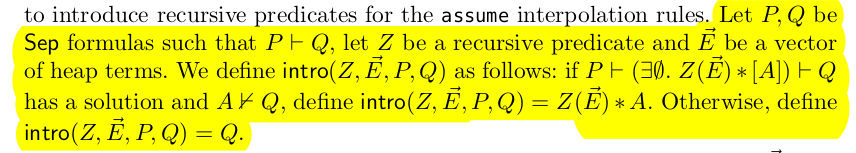
\includegraphics[scale=0.4]{24.png}
\end{center}
At last we take \texttt{itp}$(S,\texttt{c}, I')$ to be $M$, where
\begin{center}
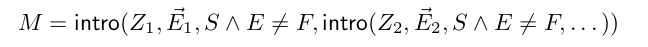
\includegraphics[scale=0.4]{25.png}
\end{center}
\end{frame}

\begin{frame}{How is Bounded Abduction Conducted}
Problem: 
$$L\vdash \exists. M \ast [A]\vdash R$$

High level description:
\begin{itemize}
\item Find a coloring of $L$, assign color red or blue to the heaplets in $L$. Red for satifying $M$, blues are left overs.
\item Compute the color strengthening $\color{red}[M']\color{black}\ast\color{blue}[A]\color{black}$ for $R$ by \color{orange} recursion on the proof of $L \vdash R$.\color{black}
\item Check $M\ast A \models R$, if failed the algorithm fails to compute the solution for the problem.
\end{itemize}

\end{frame}
\begin{frame}{Phase 3: Spatial Interpolation Modulo Theories}
\begin{center}
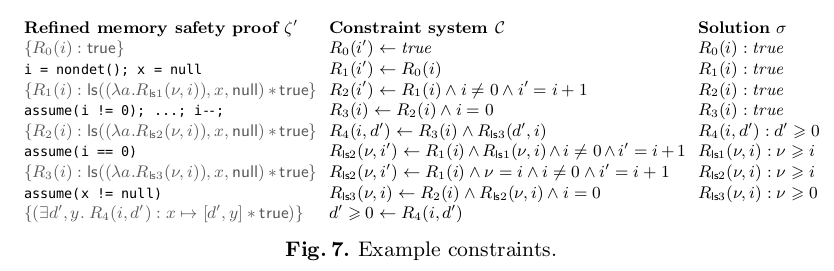
\includegraphics[scale=0.4]{26.png}
\end{center}
\end{frame}
\end{document}